\begingroup
\clearpage
\let\clearpage\relax
\vspace*{-16pt}
\chapter[DATA PREPARATION AND GRAPH CONSTRUCTION]{DATA PREPARATION AND GRAPH CONSTRUCTION}\label{sec.DATAPREP}
\endgroup

This chapter describes the data preparation steps and comorbidity
graph construction. We begin by extracting and preprocessing data from the
MIMIC-IV electronic health record database, including the mapping of
ICD diagnosis codes to higher-level disease categories. We then detail
the construction of the comorbidity graph from the preprocessed data.

We used version 3.1 of the Medical Information Mart for Intensive
Care IV (MIMIC-IV)~\citep{mimiciv}, a publicly available,
de-identified EHR repository derived from admissions to Beth Israel
Deaconess Medical Center (BIDMC) between 2008 and 2019, developed in
collaboration with MIT. MIMIC-IV contains structured data on vital
signs, laboratory measurements, medications, procedures, diagnosis
codes, and de-identified clinical notes from routine clinical care.
Access is restricted to credentialed researchers who complete human
subjects training and sign a data use agreement; the BIDMC
Institutional Review Board waived informed consent for its release.
Complete details on data acquisition, transformation, and
de-identification are provided in~\citep{mimiciv}. The database is
hosted on PhysioNet~\citep{physionet} under the MIMIC-IV project,
with separate \texttt{hosp} and \texttt{icu} modules.

Unique patient identifiers and in-hospital mortality status were
extracted from \texttt{admissions.csv} using the \texttt{subject\_id}
and \texttt{hospital\_expire\_flag} columns, respectively, where the
latter indicates whether a patient died during the hospital stay. For
patients who expired outside the hospital, mortality information was
obtained from \texttt{patients.csv} via the \texttt{dod} column,
which records each patient's date of death. All ICD-coded diagnoses
were obtained from \texttt{diagnoses\_icd.csv}; all files reside in
the \texttt{hosp} module. Following the MIMIC-IV de-identification
protocol, dates of death are censored at one year after the patient's
last hospital discharge. A null \texttt{dod} therefore indicates that
the patient was known to be alive at least one year beyond their final
encounter, while a non-null \texttt{dod} indicates death within that
window. No inferences about mortality beyond one year can be drawn.
Consequently, the mortality rate in the dataset is 16.51\%,
representing one-year post-discharge mortality across the full cohort,
and is comparable across patients regardless of when in the 2008--2019 window their last encounter occurred.

Diagnoses in MIMIC-IV are coded using both ICD-9-CM and
ICD-10-CM~\citep{cdc_icd9cm_2013, cdc_icd10cm_2022}. The transition
between coding systems, combined with the hierarchical granularity of
ICD codes---which distinguish closely related conditions by anatomy,
etiology, or clinical context---can introduce redundancy and inflate
comorbidity counts when analyzing raw codes.

To address this, all ICD-9 and ICD-10 diagnosis codes were mapped to
clinically coherent, higher-level categories using the Clinical
Classifications Software (CCS) for ICD-9 and its successor, the
Clinical Classifications Software Refined (CCSR) for
ICD-10~\citep{toolssoftware}. Developed by the Healthcare Cost and
Utilization Project (HCUP), these tools aggregate thousands of
granular ICD codes into a smaller set of mutually exclusive,
medically meaningful disease categories. This mapping reduces
duplication, improves comparability across the ICD-9/ICD-10
transition, and enhances the interpretability of comorbidity
patterns~\citep{malecki2024development}.

The full MIMIC-IV cohort contains \numprint{223291} patients, of whom
\numprint{36872} are recorded as expired. The number of diseases per patient ranges from 1 to 194, with an average of 14.12. From this cohort, we created seven subsets of \numprint{1000}, \numprint{5000}, \numprint{10000}, \numprint{15000}, \numprint{20000}, \numprint{25000}, and
\numprint{30000} patients. For each size, five independent simple
random samples without replacement were drawn, with each patient
selected uniformly at random from the complete cohort. To ensure
reproducibility while introducing variety, the five replicates for
each cohort size were generated using fixed random seeds 13, 18, 35,
66, 74, 100, and 1318. The resulting 35 sampled datasets constitute
the testbed used in all subsequent experiments.

As introduced in Section~\ref{sec.probstmnt}, each high-level disease
category (after CCS and CCSR mapping) corresponds to a vertex in the
comorbidity graph, and an undirected edge $\{u,v\}$ is included
whenever the Ochiai coefficient meets or exceeds a
threshold $\Delta$.
To select an appropriate threshold $\Delta$, we followed the
methodology of~\citet{KALGOTRA2020}, which uses the $\phi$-correlation
coefficient as a proxy for statistical significance. Given the
large sample size, we applied a significance level of $\alpha = 0.01$.
This procedure identified \numprint{8539} statistically significant
edges, corresponding to an Ochiai coefficient threshold of $\Delta = 0.1191$, which
we adopted as the edge inclusion cutoff.

The resulting comorbidity graph contains 467 vertices and
\numprint{8539} edges, with an edge density of 0.08. It consists of
one large connected component comprising 465 vertices and one small
component of 2 vertices linked by a single edge.

With the testbed established and the comorbidity graph constructed,
we turn to the computational experiments.
Chapter~\ref{sec.results} presents the results of applying the
methods developed in Chapter~\ref{sec.methods} to the complete
dataset and the 35 sampled instances derived from the MIMIC-IV
cohort, comparing their performance in terms of solution quality and
computational efficiency. The experiments cover six solution methods:
the modified Bron--Kerbosch and combinatorial branch-and-bound
algorithms, two MILP formulations, and the pure and hybrid
logic-based Benders decomposition algorithms. In addition to the
core comparisons, two side-constraint case studies are presented: an
age-based constraint and a cancer-containing constraint, both solved
using the hybrid algorithm. The chapter also includes a scalability
study on the full MIMIC-IV dataset using the size-restricted variant
and a marginal mortality rate analysis.

Figure~\ref{fig.snapshot} shows the first five rows of the prepared
dataset. The first column is the unique patient identifier. The
second column indicates the mortality status of the patient, where 1
denotes an expired patient and 0 denotes a patient who is alive. The
third column lists the disease categories with which each patient has
been diagnosed.

\begin{figure}[htbp]
    \centering
    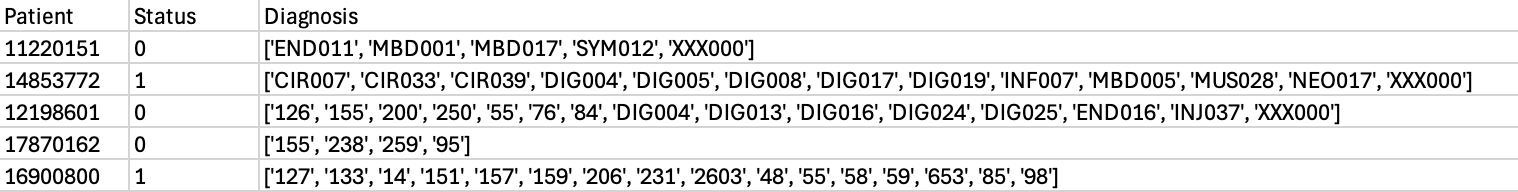
\includegraphics[width=1\textwidth]{snapshot.png}
    \caption{First Five Rows of the Prepared Dataset}
    \label{fig.snapshot}
\end{figure}